\documentclass[12pt]{article}

\usepackage[utf8]{inputenc}
\usepackage[T1]{fontenc}
\usepackage{lmodern}

\usepackage[margin=1in]{geometry}
\usepackage{parskip}

\usepackage{tikz,url,amssymb,amsmath,epsfig,color,xspace,alltt,mathtools,multirow,tikz-qtree}
\usetikzlibrary{trees}
\usepackage[pdfauthor={Brandon Fowler}]{hyperref}
\usepackage{graphicx}

\usepackage{algorithm2e}
\setlength{\algomargin}{0pt}
\DontPrintSemicolon

\usepackage{fancyhdr}
\pagestyle{fancy}

\rhead{Brandon Fowler}
\usepackage[shortlabels]{enumitem}
\setlist{nosep}

\title{Calculating Artifact Roll Outcomes}
\author{Brandon Fowler}

\begin{document}
	
\maketitle

This document provides an overview of the approach taken to calculate all possible outcomes for an artifact in Genshin Impact.

\tableofcontents
\pagebreak

\section{Sub-Stat Probability}
	
Unique combinations are computed and the probability of each corresponding permutation is calculated based on the stat weights.

The formula for the likelihood of a permutation, where $w_i$ is the weight of sub-stat $i$, is:
\begin{align*}
	\left(\frac{w_1}{Total}\right)\left(\frac{w_2}{Total - w_1}\right)\left(\frac{w_3}{Total - w_1 - w_2}\right)\dots
\end{align*}

For a given unique combination, all of these probabilities are added together for all permutations that correspond to that unique combination.

The sub-stat probability is then the sum of probabilities of combinations that are valid given the inputted constraints,
\begin{align*}
	SubstatProbability = \sum_{valid} p
\end{align*}
	
\section{Roll Probability}

The probability for a given sub-stat outcome is:
\begin{align*}
	p\left(\frac{1}{InitialValueOutcomes}\right)\left(\frac{1}{RollOutcomes}\right)\left(\frac{1}{RollValueOutcomes}\right)
\end{align*}

Where:
\begin{itemize}[]
	\item $p$ is the probability of the stat combination.
	\item $InitialValueOutcomes$ the number of value outcomes for the initial states.
	\item $RollOutcomes$ is the number of possible roll outcomes.
	\item $RollValueOutcomes$ the number of value outcomes for the rolled stats.
\end{itemize}

Since the sub-stat probability is separately defined above, we have:
\begin{align*}
	&\begin{aligned}[t]Roll&Probability \times SubstatProbability = \\
	&p\left(\frac{1}{InitialValueOutcomes}\right)\left(\frac{1}{RollOutcomes}\right)\left(\frac{1}{RollValueOutcomes}\right)\end{aligned} \\[12pt]
	&\begin{aligned}[t]Roll&Probability \times \sum_{valid} p = \\
	&p\left(\frac{1}{InitialValueOutcomes}\right)\left(\frac{1}{RollOutcomes}\right)\left(\frac{1}{RollValueOutcomes}\right)\end{aligned} \\[12pt]
	&\begin{aligned}[t]Roll&Probability = \\
	&\left(\frac{p}{\sum_{valid} p}\right)\left(\frac{1}{InitialValueOutcomes}\right)\left(\frac{1}{RollOutcomes}\right)\left(\frac{1}{RollValueOutcomes}\right)\end{aligned}
\end{align*}

\pagebreak
Let:
\begin{itemize}[]
	\item $a$ - The number of sub-stats
	\item $a_{r}$ - The number of rollable sub-stats
	\item $b$ - The number of roll values
	\item $n$ - The number of sub-stat rolls
\end{itemize}

Then, there are $a = 4$ sub-stats to roll initially, $a^* = 4$ sub-stats choose from each time for each roll, and $b = 4$ roll values a roll can have (70\%, 80\%, 90\%, and 100\%).
\begin{itemize}[]
	\item $InitialValueOutcomes = b^a = 4^4$ - There are 4 sub-stats to assign base values to
	\item $RollOutcomes = a_{r}^n = 4^n$ - There are $n$ sub-stats rolls that each choose a sub-stat
	\item $RollValueOutcomes = b^n = 4^n$ - The $n$ sub-stats rolls needs value assigned
\end{itemize}

Thus, the total number of possibilities is:
\begin{align*}
	(b^a)(a_{r}b)^n = (4^4)(16^n)
\end{align*}

\subsection{Roll Permutations}

To preserve the base of 4, each guaranteed roll is counted as $\frac{4}{\# of guaranteed rolls} = \frac{4}{2} = 2$.

To reduce computation, the computed $4^n$ roll permutations are combined into combinations, giving each effective outcome a value $RollPermutations$.

\subsection{Roll Values}

For each of these, the number of good outcomes is found based on the possible roll values.

For $n$ rolls, there are $4^{a+1}4^{b+1}4^{c+1}4^{d+1}$ possible roll value combinations where $a + b + c + d = n$.

A method computes the roll value distribution of $x = a+1, \dots, d+1$. It iterates $x$ times, considering the 4 possible roll values that can extend the current computed values each time. To avoid computing a full $4^x$ outcomes, after each stage, paths with the same value are combined.

For example, assume the roll values are 0, 0.5, and 1. After the second iteration, we have:

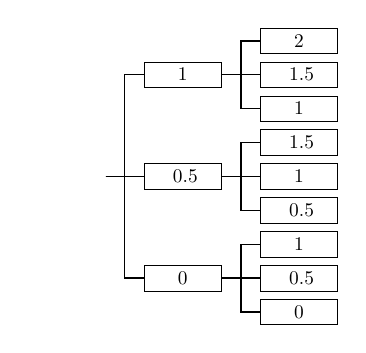
\begin{tikzpicture}[level distance=6em,sibling distance=0.4em,scale=.7]
	\tikzset{edge from parent/.style= 
		{thick, draw,
			edge from parent fork right},every tree node/.style={draw,minimum width=4em,text width=1em, align=center},grow'=right}
	\Tree 
	[.\node[draw=none]{}; 
	[.1
	[.2 ]
	[.1.5 ]
	[.1 ]
	]
	[.0.5
	[.1.5 ]
	[.1 ]
	[.0.5 ]
	] 
	[.0
	[.1 ]
	[.0.5 ]
	[.0 ]
	]
] 
\end{tikzpicture}

Giving us $3^2 = 9$ outcomes to bring to the next iteration.

But instead, they can be grouped as so: 2 (1x), 1.5 (2x), 1 (3x), 0.5 (2x), 0 (1x). This leaves only 5 outcomes to bring to the next iteration. This is repeated for all of the $x$ iterations.

The general method to compute the number of outcomes above the goal also uses this method, but for the $4$ stat iterations.

This gives each outcome $RollValuePossibilities_i$ for $i = 1, \dots, 4$.

\subsection{Total Probability}

The probability associated with a single outcome is now:
\begin{align*}
	\frac{p \times RollPermutations \times \prod_{j = 1}^{4} RollValuePossibilities_j}{\sum_{valid} p \times RollOutcomes \times InitialValueOutcomes \times RollValueOutcomes}
\end{align*}

So, the total probability is:
\begin{align*}
	Tot&alProbability \\[8pt]
	&= \sum_{i = 1}^{|combos|}\left(\frac{p \times RollPermutations \times \prod_{j = 1}^{4} RollValuePossibilities_j}{\sum_{valid} p \times RollOutcomes \times InitialValueOutcomes \times RollValueOutcomes}\right) \\[12pt]
	&= \frac{\sum_{i = 1}^{|combos|} p_i \times RollPermutations_i \times \prod_{j = 1}^{4} RollValuePossibilities_{i,j}}{\sum_{valid} p \times RollOutcomes \times InitialValueOutcomes \times RollValueOutcomes} \\[12pt]
	&= \frac{\sum_{i = 1}^{|combos|} p_i \times RollPermutations_i \times \prod_{j = 1}^{4} RollValuePossibilities_{i,j}}{\sum_{valid} p \times (4^n)^2(4^4)}
\end{align*}

\subsection{Generating Outcomes}

An overview of the code used to generate all outcomes is thus:

\begin{algorithm}[H]
	\SetInd{0.4em}{0.4em}

	Sum = 0 \\
	
	\ForEach{$(s_1, s_2, s_3, s_4 \rightarrow p)$ of GenerateCombos}{
		\ForEach{$(r_1, r_2, r_3, r_4 \rightarrow RollPermutations)$ of RollCountsDist}{
			States = Map($0 \rightarrow 1$) \\
			
			\For{$i = 1 \dots 4$}{
				NextStates = Map() \\
				
				\ForEach{$(State \rightarrow Ways)$ of States}{
					\ForEach{($statSum_i \rightarrow RollValuePossibilities_i$) of ValueOfRollsDist($r_i + 1$)}{
						NextState = $State + statSum_i \times weight_i$ \\
						NextStates[$NextState$] += $Ways \times RollValuePossibilities_i$
					}
				}
				
				States = NextStates
			}
			
			\ForEach{$(State \rightarrow Ways)$ of States}{
				\If{$State$ is within goal}{
					Sum += $p \times RollPermutations \times Ways$
				}
			}
		}
	}
	
	\Return $Sum \div (\sum_{valid} p \times (4^4)(4^n)^2))$
\end{algorithm}

Note that at the end, $Ways$ is just the product of the $RollValuePossibilities_i$, $i = 1, \dots, 4$, for the outcome.

The distribution viewer provides a way to visualize $RollCountsDist$ and $ValueOfRollsDist$.

\subsection{Varying Initial Stat Count}

Since artifacts have a chance to have 4 or 5 rolls (corresponding to 3 or 4 initially enabled stats), the actual probability is,
\begin{align*}
	TotalProbability_{n=4} \times (1 - P(n = 5)) + TotalProbability_{n=5} \times P(n = 5)
\end{align*}

So, the above pseudo-code is called twice for each calculation.

\end{document}